\begin{problem}{竹叶狂想曲}{竹叶狂想曲.in}{竹叶狂想曲.out}{1 seconds}


话说回来,四月份都已经够热了,时值五月份的今天更是热得让人受不了,而且湿气也更重,一再挑动着我的不快指数。上海理工大学廉价的校舍,跟空调之类的高级机械可以说是完全无缘。综合楼的教室简直就像前往灼热地狱的候车室一样,我确信设计者一点居住舒适环境的概念都没有。

一个我熟识的人紧贴在操场门前。我一眼就看出正作势要爬上铁门的娇小人影。

紧贴在门上、回过头来的那张脸,确实比我所认识的SOS团团长来得年幼。但是那双绝对不会错认的眼睛中的光芒,不折不扣就是春日的眼神。即使她是一身T恤配上短裤的轻松打扮,这种印象依然没有什么改变。三年前的现在,春日是国中一年级的学生。

“你是什么人?变态?还是绑架犯?看起来真是可疑。”

朦胧的街灯将四周照得微微发白。我没办法看清楚春日细部的表情,但是还在念国中一年级的春日的眼神,很明显地变成看着可疑人物的色彩。三更半夜企图溜进操场的女孩子,和一个刚刚结束996在校园路上徘徊的我,哪一个比较可疑?我实在不想深入去思考这个问题。

“你才可疑。你在这里干什么?”

“那还用说?当然是非法入侵。”

别这么冠冕堂皇地宣扬自己的犯罪行为。恼羞成怒也要有个限度。

“你来得正好。我虽然不认识你,但是要是你有空的话,就帮我一下忙吧。“ 

她竟然可以这样脸不红、气不喘地,对一个素昧平生的大学生颐指气使,果然是如假包换的春日。要是我第一次遇见这种国中女生的话,我大概会认为她是危险的神经病吧?

幸运的是,我还有别的人可以依靠。没错没错,就是盯着电脑屏幕看的你,这个烂摊子就交给你了!

春日想要你帮忙拿石灰粉划线机在操场上划线,当然你只能乖乖的听她指手画脚咯。


\InputFile

第一行一个正整数 $n (1 \leq n \leq 10^5)$ ,表示春日命令的数量。

接下来 $n$ 行,每行包含至少一个正整数 $op_i \in \{ 1,2,3,4 \}$ ,表示春日第 $i$ 个命令的种类。

如果 $op_i==1$ ,接下来会有四个正整数 ${X1}_i,{Y1}_i,{X2}_i,{Y2}_i$ ,表示春日想要画一条端点分别在 $({X1}_i,{Y1}_i)$ 和 $({X2}_i,{Y2}_i)$ 的线段,保证春日不会想要画一个点。

如果 $op_i==2$ ,接下来会有一个正整数 $X_i$ ,表示需要回答春日"与直线 $X=X_i$ 有公共点的线段的数量"。

如果 $op_i==3$ ,接下来会有一个正整数 $Y_i$ ,表示需要回答春日"与直线 $Y=Y_i$ 有公共点的线段的数量"。

如果 $op_i==4$ ,表示春日想要擦掉最近画的一条线段。(如果没有线条可擦那你就无视她的这个命令)

约定所有的整数满足 $1 \leq x \leq 10^6$ 。

\OutputFile

对于每一个询问,输出一行一个整数表示回答。

\Example

\begin{example}
\exmp{
15 
1 2 2 2 8
1 4 2 6 8
1 8 2 6 8
1 5 5 7 5
1 9 2 9 8
1 9 5 12 2
1 9 5 12 8
1 14 2 14 8
1 16 2 16 8
1 19 2 19 8
1 16 2 19 2
1 16 8 19 8
1 21 2 21 8
3 3
2 6
}{
9
3
}%
\end{example}
\begin{center}
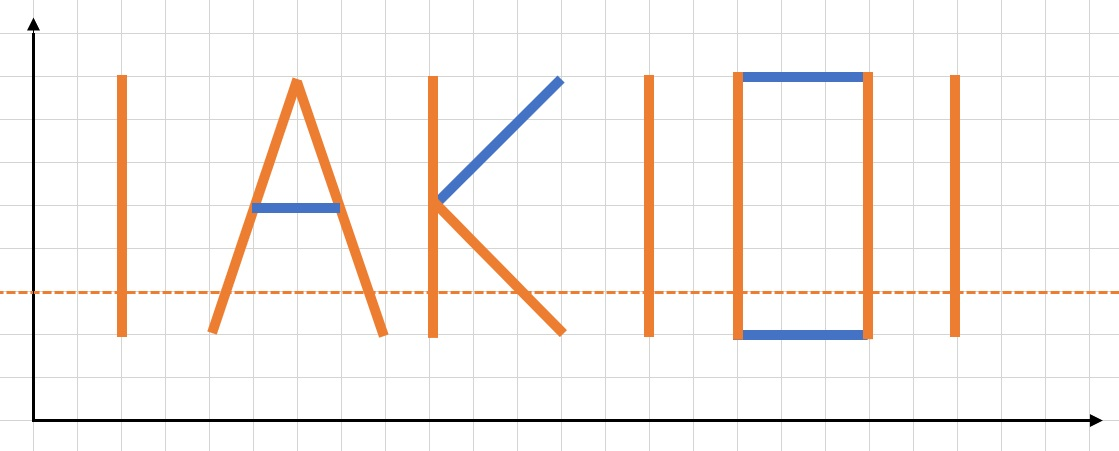
\includegraphics[width=0.8\textwidth]{pics/D.jpg}
\end{center}
样例的第一个询问如图所示
\end{problem}
